\section{ADD-L: A New Probabilistic Representation}
\label{sec:ADDL}

In order to compute the Shannon entropy of a circuit formula $\varphi(X, Y)$, we need to use the probability distribution over the outputs.
Algebraic Decision Diagrams (ADDs) are an influential compact probability representation that can be exponentially smaller than the explicit representation.
Macii and Poncino~\cite{macii1996exact} showed that ADD supports efficient exact computation of entropy.
However, we observed in the experiments that the sizes of ADDs often exponentially explode with large circuit formulas.
We take inspiration from a Boolean representation called Ordered Binary Decision Diagram with implied Literals (OBDD-L)~\cite{lai2013reduced}, which reduces its size by recursively extracting implied literals and can be exponentially smaller than the original OBDD.
Accordingly, we propose a probabilistic representation called Algebraic Decision Diagrams with implied Literals (ADD-L) and show it supports tractable entropy computation.
ADD-L is a general form of ADD and is defined as follows:

\begin{definition}\label{ADDL-definition}
An ADD-L is a rooted DAG, where each node $u$ is either terminal or non-terminal.
Each terminal node $u$ is labeled with a real weight $\omega(u)$ and a set of implied literals $L(u)$.
Each non-terminal node $u$ is associated with a variable $\mathit{var}(u)$, two children, and a set of implied literals $L(u)$, which satisfies that $\mathit{var}(u)$ does not appear in $L(u)$ and that each variable appearing in $L(u)$ does not appear in the descendants of $u$.
The children of non-terminal node $u$ are referred to as the \textit{low} child $lo(u)$ and the \textit{high} child $hi(u)$, and connected by dashed lines and solid lines, respectively, corresponding to the cases where $\mathit{var}(u)$ is assigned the value of $\mathit{false}$ and  $\mathit{true}$. 
An ADD-L is imposed with a linear ordering $\prec$ of variables such that given a node $u$ and its non-terminal child $v$, $\mathit{var}(u) \prec \mathit{var}(v) $.
\end{definition}

Hereafter, we denote to the set of variables that appear in $v$ (i.e., the variables in $\mathit{var}(v)$ and $L(v)$ as well as all the variables that appear in its descendant nodes) as $\mathit{Vars}(v)$.
It is obvious that when each set of implied literals is empty, an ADD-L is equivalent to an ADD.
%In our experiments, we observed that given a large circuit formula, the assignment of a decision variable often results in a large number of implied literals, and therefore the ADD-L often has a much smaller size than the corresponding ADD.
In our experiments, we observed that given a large circuit formula, assigning a decision variable often results in a large number of implied literals, and therefore, the ADD-L often has a much smaller size than the corresponding ADD.
We now turn to show that how an ADD-L defines a probability distribution:
 
\begin{definition}\label{def:ADDL-weight}
	Let $u$ be an ADD-L node over a set of variables $Y$ and let $\sigma$ be an assignment over $Y$. 
    The weight of $\sigma$ is defined as follows:
	\begin{equation*}
	   \omega(\sigma,u) =  
	   \begin{cases}  
    	   0 & \sigma \not\models L(u) \\  
		   \omega(u) & \text{$u$ is terminal and $\sigma \models L(u)$} \\  
            \omega(\sigma,lo(u)) & \text{$u$ is non-terminal and $\sigma \models L(u) \cup \{\lnot \mathit{var}(u)\}$}  \\
            \omega(\sigma,hi(u)) & \text{$u$ is non-terminal and $\sigma \models L(u) \cup \{\mathit{var}(u)\}$}  \\
	   \end{cases}  
	\end{equation*}
    The weight of an non-constant ADD-L rooted at $u$ is denoted by $\omega(u)$ and defined as $\sum_{\sigma \in 2^{\mathit{Vars}(u)}}\omega(\sigma,u)$.
    The probability of $\sigma$ over $u$ is defined as $p(\sigma, u) = \frac{\omega(\sigma,u)}{\omega(u)}$.
\end{definition}

Figure \ref{fig:ADDL-example1} depicts an ADD-L to represent the probability distribution of the circuit formula in Example \ref{circuit-example} over its outputs.
Let $u$ be its root and let $\sigma = \{y_1 \mapsto \mathit{false}, y_2 \mapsto \mathit{false}, y_3 \mapsto \mathit{false}\}$.
By Definition \ref{def:ADDL-weight}, $\omega(\sigma, u) = 2$, $\omega(u) = 7$, and $p(\sigma, u) = \frac{2}{7}$.
\begin{figure}[!htbp]
	
	\centering
	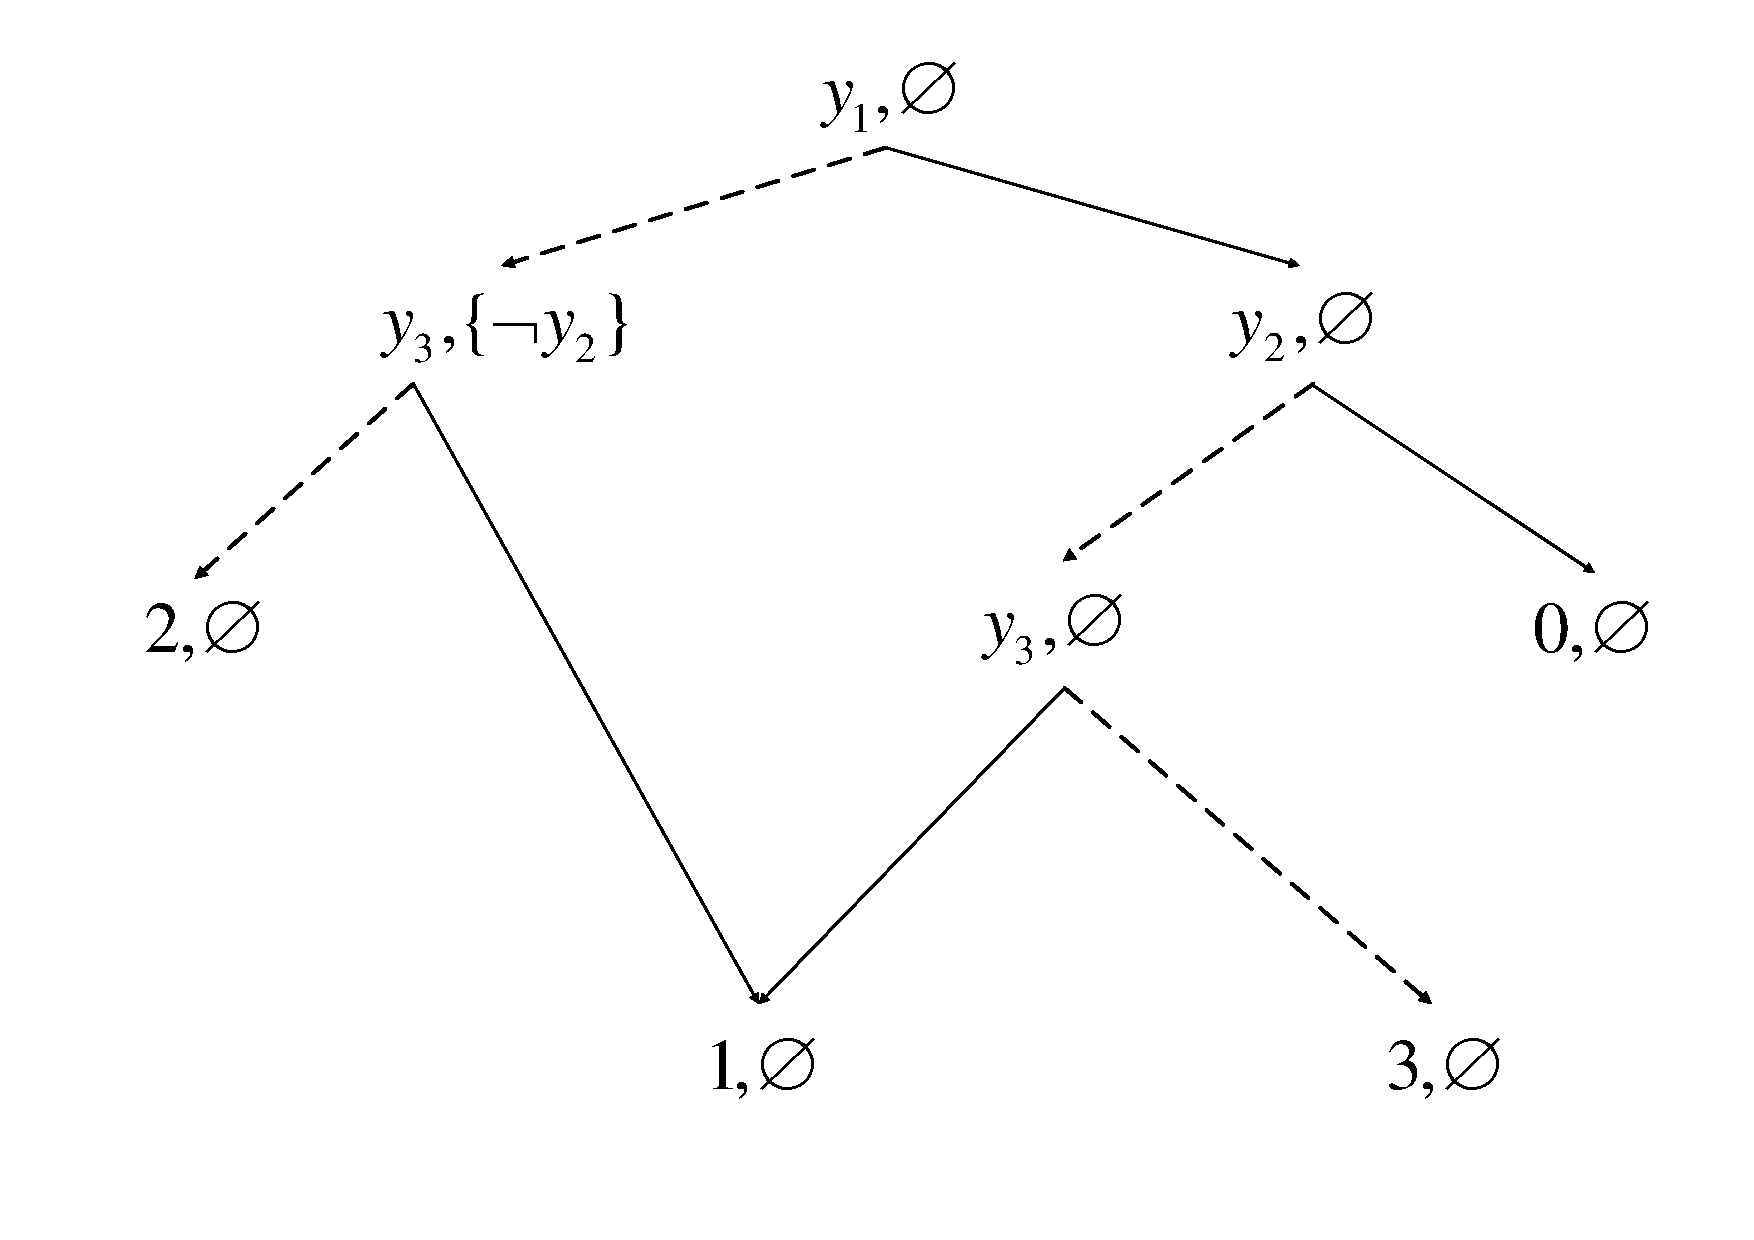
\includegraphics[width=0.7\linewidth]{figures/ADD-L-example1.pdf}
	\caption{An ADD-L example corresponding to Example \ref{circuit-example}, where the weight of a terminal node is the model count of $\varphi[\sigma]$ ($\sigma$ is a partial assignment corresponding to the decisions on a path from the root to it)}
	\label{fig:ADDL-example1}
\end{figure}

\subsection{Tractable Computation of Weight and Entropy}
	%\left| \mathit{Sol}(\varphi(Y \mapsto \sigma)) \right| & \text{$u$ is terminal node and $\sigma \models L(u)$} \\ 
	
	The computation of Shannon entropy of ADD-L depends on the computation of its weight. 
    We first show that for an ADD-L node $u$, we can compute $\omega(u)$ in polynomial time.
	\begin{proposition}\label{prop:omega-proposition}
		Given a non-terminal node $u$ in ADD-L, its weight $\mathit{\omega}(u)$ can be recursively computed as follows in polynomial time:
		$$\mathit{\omega}(u) = 2^{n_0} \cdot \mathit{\omega}(lo(u)) + 2^{n_1} \cdot \mathit{\omega}(hi(u))$$
		where $n_0 = |\mathit{Vars}(u)| - |\mathit{Vars}(lo(u))|-1 - |L(u)|$ and $n_1 = |\mathit{Vars}(u)| - |\mathit{Vars}(hi(u))|-1 - |L(u)|$. 
		%The model counting of the formula represented by $u$ satisfies $CT(u) = \mathit{\omega}(u)$.
		
		\begin{proof}
            The time complexity is immediate by using dynamic programming.
            We prove the equation can compute the weight correctly by induction on the number of variables of the ADD-L rooted at $u$.
            It is obvious that the weight of a terminal node is the real value labeled. 
            Assume that when $|\mathit{Vars}(u)| \le n$, this proposition holds. 
            For the case where $|\mathit{Vars}(u)| = n + 1$, we use $Y_0$ and $Y_1$ to denote $\mathit{Vars}(lo(u))$ and $\mathit{Vars}(hi(u))$, and we have $|Y_0| \le n$ and $|Y_1| \le n$.
            Thus, $\mathit{\omega}(lo(u))$ and $\mathit{\omega}(hi(u))$ can be computed correctly.
            According to Definition \ref{def:ADDL-weight}, $w(u) = \sum_{\sigma \in 2^{\mathit{Vars}(u)}}\omega(\sigma,u)$.
            The assignments over $\mathit{Vars}(u)$ can be divided into three categories: 
            \begin{itemize}
              \item The assignment $\sigma \not\models L(u)$: $\omega(\sigma, u) = 0$.
              \item The assignment $\sigma \models L(u) \cup \{\lnot \mathit{var}(u)\}$: 
              It is obvious that $\omega(\sigma, u) = \omega(\sigma_{\downarrow Y_0}, lo(u))$. 
              Each assignment over $Y_0$ can be extended to exactly $2^{n_0}$ different assignments over $\mathit{Vars}(u)$ in this category. Thus, we have the following equation:
              $$\sum_{\sigma \in 2^{\mathit{Vars}(u)} \land \sigma \models L(u) \cup \{\lnot \mathit{var}(u)\}}\omega(\sigma, u) = 2^{n_0} \cdot \mathit{\omega}(lo(u)).$$
              \item The assignment $\sigma \models L(u) \cup \{\mathit{var}(u)\}$: This case is similar to the above case.
            \end{itemize}
            To sum up, we can obtain that $\mathit{\omega}(u) = 2^{n_0} \cdot \mathit{\omega}(lo(u)) + 2^{n_1} \cdot \mathit{\omega}(hi(u))$.	
		\end{proof}
		
	\end{proposition}
	
	Now we explain how ADD-L computes its Shannon entropy in polynomial time.
	\begin{proposition}\label{prop:Entropy-proposition}
		Given an ADD-L rooted at $u$, we use $\mathit{infor}(v)$ to denote the self-information of the subgraph rooted at $v$.
		We can recursively compute $\mathit{infor}(v)$ in polynomial time as follows:
		\begin{equation*}
		\mathit{infor}(v) =  
		\begin{cases}  
			-\frac{\omega(v)}{\omega(u)} \cdot \log \frac{\omega(v)}{\omega(u)} & v \ is \ terminal   \\
			2^{n_0} \cdot \mathit{infor}(lo(u)) + 2^{n_1} \cdot \mathit{infor}(hi(u)) & otherwise
			
			%-\frac{\omega(v)}{\omega(u)} \cdot \log \frac{\omega(v)}{\omega(u)} \cdot 2^{|Vars(u)| - |Vars(v)|} & v \ is \ terminal   \\
			%\frac{\mathit{infor}(lo(u)) + \mathit{infor}(hi(u))}{2^{ |L(u)| + 1}} & otherwise
			
		\end{cases}  
		\end{equation*}
        where $n_0 = |\mathit{Vars}(v)| - |\mathit{Vars}(lo(v))|-1 - |L(v)|$ and $n_1 = |\mathit{Vars}(v)| - |\mathit{Vars}(hi(v))|-1 - |L(v)|$.  
        The entropy of the probability distribution represented by $u$ satisfies $H(u) = \mathit{infor}(u)$.
		
		
		\begin{proof}
        According to Proposition \ref{prop:omega-proposition}, $\omega(u)$ can be computed in polynomial time, and therefore the time complexity in this proposition is obvious.
		According to Definition \ref{def:ADDL-weight}, $H(u) = -\sum_{\sigma \in 2^{\mathit{Vars}(u)}}\frac{\omega(\sigma,u)}{\omega(u)}\log\frac{\omega(\sigma,u)}{\omega(u)}$.
		We modify the weight of each terminal node $v$ in the ADD-L rooted at $u$ as $-\frac{\omega(v)}{\omega(u)} \cdot \log \frac{\omega(v)}{\omega(u)}$ and assume that the root of the new ADD-L is $u'$.
        It is obvious that $\omega(u') = \mathit{infor}(u)$.
        According to Proposition \ref{prop:omega-proposition}, we know the equation in this proposition can compute $\omega(u')$ correctly.
        Then this proposition holds due to the fact $H(u) = \omega(u')$.
		\end{proof}
		
	\end{proposition}
	
We close this section by explaining why we use the orderedness in the design of ADD-L.
Actually, Propositions \ref{prop:omega-proposition}--\ref{prop:Entropy-proposition} still hold when we only use the more general read-once property: each variable appears at most once in each path from the root of an ADD-L to a terminal node.
First, we observed in our experiments that the linear ordering given by minfill in our tool PSE works better than the dynamic orderings in the state-of-the-art model counters, where the former imposes the orderedness and the latter imposes the read-once property.
Second, ADD-L can provide tractable equivalence checking between probability distributions beyond this study.
